\begin{frame}{Atribuição Estática Única}
    \begin{itemize}
        \item A forma de atribuição estática única (do inglês, \textit{static single assignment}, ou SSA) representa uma particularidade de CFG.

        \item Para estar nesse formato, é estabelecido que cada referência a uma variável esteja vinculada a uma única atribuição.

        \item É necessário, então, realizar um procedimento de renomeação de todas as variáveis com mais de uma atribuição no código base.
    \end{itemize}
\end{frame}

\begin{frame}{SSA - Exemplos}
    \begin{figure}
        \centering
        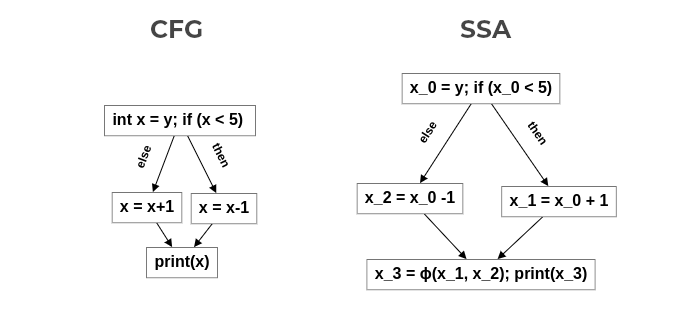
\includegraphics[width=.9\textwidth]{Figuras/ssa-cfg.png}
        \caption{Passagem de CFG para SSA}
        \label{fig:cfg-ssa}
    \end{figure}
\end{frame}

\begin{frame}{Funções $\phi$}
    \begin{itemize}
        \item As funções $\phi$ são funções de decisão que, ao receber como entrada as atribuições provenientes de diferentes arestas que fluem para um mesmo bloco, determinam qual valor utilizar.

        \item Para gerar uma representação SSA eficiente, é necessário que as funções $\phi$ sejam colocadas somente onde são necessárias, pois o excesso destas funções aumenta o custo de qualquer algoritmo que precise percorrer grafo na forma SSA.

        \item Uma estratégia para auxiliar o algoritmo na criação da forma SSA com um número menor de funções $\phi$ é realizar uma análise de dominância entre os blocos.
    \end{itemize}
\end{frame}

\begin{frame}{Análise de Dominância}
    \begin{itemize}
        \item Tabela de dominância: representada por $D_{OM}(n)$, onde $m\in D_{OM}(n)$ se, para alcançar $n$ é \textit{necessário} passar por $m$; e dominante imediato, indicado por $ID_{OM}(n)$, tal que se $m\in D_{OM}(n)$ e $m$ é o nó mais próximo de $n$ neste conjunto, com $m \neq n$, então $m$ é o dominante imediato de $n$. Se $m \in D_{OM}(n)$ e $m\neq n$ então dizemos que $m$ domina estritamente $n$, denotado por $m\gg n$.
        \item[] 

        \item Tabela de Fronteira de Dominância: 
        \begin{equation}
            \begin{matrix}
                DF(n) = \{m | (\exists P \in Pred(m)) & (n \in D_{om}(P) & e & n \not\gg m)\}
            \end{matrix}
        \end{equation}
    \end{itemize}

\end{frame}
